% !TEX root = ../tex/4-1.tex
% 第4章：本文は青、補足は緑
\newcommand{\asmain}{%
    \setbeamercolor{frametitle}{fg=white,bg=main}%
    \setbeamercolor{structure}{fg=main}%
    \setbeamercolor{itemize item}{fg=main}%
    \setbeamercolor{itemize subitem}{fg=main}%
    \setbeamercolor{enumerate item}{fg=main}%
}
\newcommand{\assuppl}{%
    \setbeamercolor{frametitle}{fg=white,bg=examplecol}%
    \setbeamercolor{structure}{fg=examplecol}%
    \setbeamercolor{itemize item}{fg=examplecol}%
    \setbeamercolor{itemize subitem}{fg=examplecol}%
    \setbeamercolor{enumerate item}{fg=examplecol}%
}
% フレームタイトルの「補足」だけを□で囲む
\newcommand{\supplmark}{%
    \setlength{\fboxsep}{1.5pt}%
    \setlength{\fboxrule}{0.7pt}%
    \fbox{\textbf{補足}}%
}
\asmain


%=============================================
\begin{frame}{第3章から第4章へ}
    \begin{block}{ここまで（第3章）}
        NCSNは複数ノイズの離散はしごでスコアを学び、\\
        Annealed Langevinで高$\sigma\to$低$\sigma$と生成する。\\
        DDPMも離散ステップの前向き／逆向き過程である。
    \end{block}
    \begin{block}{ここから（4.1）}
        ノイズレベルを連続時間$t\in[0,T]$に広げ、\\
        前向き過程をSDE、生成を逆時間SDE／PF-ODEとして定式化する。\\
        鍵は時間依存スコア$\nabla_{\bm{x}}\log p_t(\bm{x})$である。
    \end{block}
\end{frame}
%=============================================
\asmain
\begin{frame}{4.1 の位置づけ}
    \begin{block}{この節の役割}
        離散のはしごを連続化し、前向き・逆向き・確定的流を一本の枠にまとめる
    \end{block}
    \begin{enumerate}
        \item \textbf{動機}\\
        NCSN／DDPMの離散更新$\to$共通形$\to$前向きSDE
        \item \textbf{前向きSDE}\\
        データ$\to$ノイズ（式4.1.3）。周辺$p_t$を定義する
        \item \textbf{逆時間SDE}\\
        スコア補正でノイズ$\to$データ（式4.1.6）
        \item \textbf{PF-ODEと周辺の一致}\\
        同じ$\{p_t\}$を確率的／確定的に辿る（論文4.2の要点）
    \end{enumerate}
\end{frame}
%=============================================
\section{動機：離散から連続へ}
\asmain
\begin{frame}{区切り：動機（離散$\to$連続）}
    \tableofcontents[currentsection]
\end{frame}
%=============================================
\asmain
\begin{frame}{図4.1：時間依存のスコア場}
    \centering
    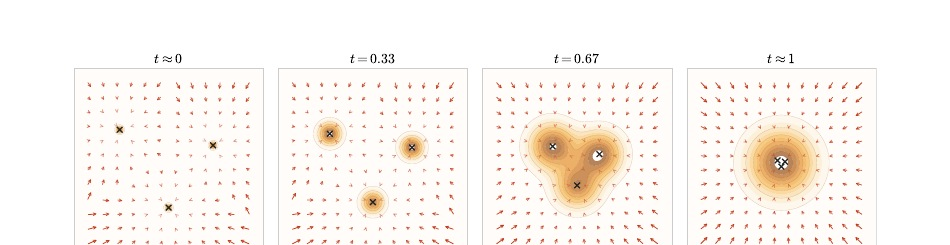
\includegraphics[width=\textwidth,height=0.62\textheight,keepaspectratio]{fig-4-1.jpg}
    \vfill
    \footnotesize
    ノイズが増えると$p_t$は多峰$\to$単峰へ。\\
    スコア$\nabla_{\bm{x}}\log p_t$は局所的な引き寄せから、大域的な中心向きへ変わる。
\end{frame}
%=============================================
\assuppl
\begin{frame}{\supplmark：図4.1の読み方}
    \begin{columns}[T,onlytextwidth]
        \begin{column}{0.48\textwidth}
            \begin{exampleblock}{$t\approx 0$}
                モード近傍に鋭い場。\\
                近くの峰へ強く引き戻す。
            \end{exampleblock}
        \end{column}
        \begin{column}{0.48\textwidth}
            \begin{exampleblock}{$t\approx 1$}
                平滑な単峰。\\
                全体の重心へ穏やかに向く。
            \end{exampleblock}
        \end{column}
    \end{columns}
    \vspace{0.4em}
    \begin{exampleblock}{Score SDEの学習対象}
        この時間依存スコアの族を学ぶことが、\\
        生成＝微分方程式を解く、という問題設定になる。
    \end{exampleblock}
\end{frame}
%=============================================
\asmain
\begin{frame}{NCSNとDDPMの離散ノイズ注入}
    NCSN：増加列$\{\sigma_i\}$で
    \[
        \bm{x}_{\sigma_i}=\bm{x}_0+\sigma_i\bm{\epsilon}_i,
        \qquad
        \bm{\epsilon}_i\sim\mathcal{N}(\bm{0},\bm{I})
    \]
    DDPM：分散スケジュール$\{\beta_i\}$で
    \[
        \bm{x}_i=\sqrt{1-\beta_i}\,\bm{x}_{i-1}+\sqrt{\beta_i}\,\bm{\epsilon}_i
    \]
    \begin{block}{見方}
        どちらも「少しずつノイズを足す」離散更新である。\\
        連続極限では同じ構造のSDEに乗る。
    \end{block}
\end{frame}
%=============================================
\asmain
\begin{frame}{共通の1ステップ形}
    離散時刻での更新はおおむね
    \[
        \bm{x}_{t+\Delta t}
        \approx
        \bm{x}_t
        +
        \bm{f}(\bm{x}_t,t)\,\Delta t
        +
        g(t)\sqrt{\Delta t}\,\bm{\epsilon}_t
        \tag{4.1.1}
    \]
    \begin{columns}[T,onlytextwidth]
        \begin{column}{0.48\textwidth}
            \begin{block}{NCSN}
                $\bm{f}=\bm{0}$，\\
                $g(t)=\sqrt{\dfrac{d\sigma^{2}(t)}{dt}}$
            \end{block}
        \end{column}
        \begin{column}{0.48\textwidth}
            \begin{block}{DDPM}
                $\bm{f}=-\dfrac12\beta(t)\bm{x}$，\\
                $g(t)=\sqrt{\beta(t)}$
            \end{block}
        \end{column}
    \end{columns}
\end{frame}
%=============================================
\asmain
\begin{frame}{図4.2：離散のノイズ追加ステップ}
    \centering
    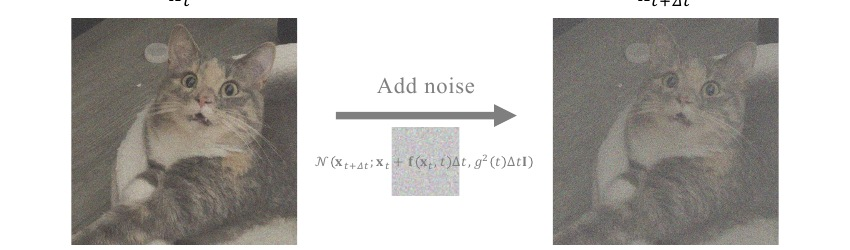
\includegraphics[width=\textwidth,height=0.58\textheight,keepaspectratio]{fig-4-2.jpg}
    \vfill
    \footnotesize
    遷移は
    $\mathcal{N}\bigl(\bm{x}_{t+\Delta t};\,
    \bm{x}_t+\bm{f}\Delta t,\,g^{2}(t)\Delta t\,\bm{I}\bigr)$
    （式4.1.2）。
\end{frame}
%=============================================
\asmain
\begin{frame}{$\Delta t\to 0$で前向きSDEへ}
    \[
        d\bm{x}(t)
        =
        \bm{f}(\bm{x}(t),t)\,dt
        +
        g(t)\,d\bm{w}(t)
    \]
    対応の読み方：
    \begin{itemize}
        \item $\bm{x}(t+\Delta t)-\bm{x}(t)\approx d\bm{x}(t)$
        \item $\Delta t\approx dt$
        \item $\sqrt{\Delta t}\,\bm{\epsilon}_t\approx d\bm{w}(t)$
        （$d\bm{w}(t)\sim\mathcal{N}(\bm{0},dt\,\bm{I})$）
    \end{itemize}
    \begin{block}{要点}
        ドリフト$\bm{f}$と拡散$g$を決めれば前向き過程は確定する。\\
        逆過程に残る未知は、各時刻のスコアだけである。
    \end{block}
\end{frame}
%=============================================
\asmain
\begin{frame}{動機のまとめ}
    \begin{itemize}
        \item 複数ノイズのはしごは、連続時間のスコア場へ一般化できる
        \item NCSN／DDPMの1ステップは共通形（4.1.1）に乗る
        \item $\Delta t\to 0$で前向きSDEになり、生成は逆過程の数値積分になる
    \end{itemize}
    \begin{block}{次}
        前向きSDEが誘導する摂動核と周辺$p_t$を書く。
    \end{block}
\end{frame}
%=============================================
\section{前向きSDE}
\asmain
\begin{frame}{区切り：前向きSDE}
    \tableofcontents[currentsection]
\end{frame}
%=============================================
\asmain
\begin{frame}{図4.3：データからノイズへ}
    \centering
    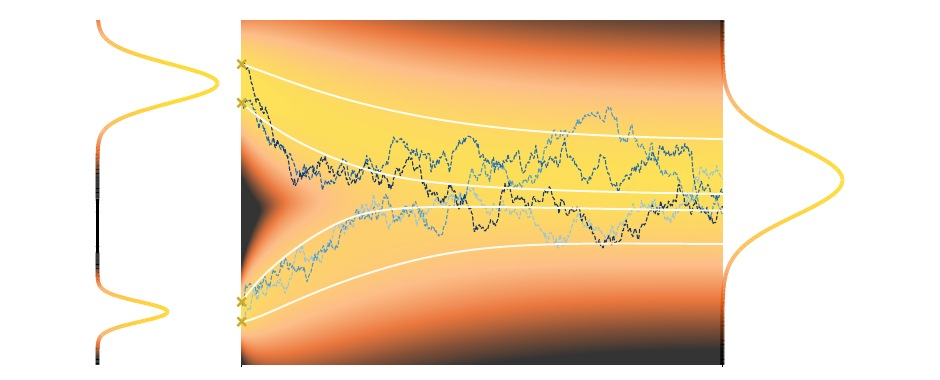
\includegraphics[width=\textwidth,height=0.62\textheight,keepaspectratio]{fig-4-3.jpg}
    \vfill
    \footnotesize
    青：確率的な前向きSDE軌跡。白：同じ周辺を辿るPF-ODE。\\
    背景は周辺密度$p_t$の時間発展。
\end{frame}
%=============================================
\asmain
\begin{frame}{前向きSDEの定義}
    $[0,T]$上の確率過程
    \[
        d\bm{x}(t)
        =
        \bm{f}(\bm{x}(t),t)\,dt
        +
        g(t)\,d\bm{w}(t),
        \qquad
        \bm{x}(0)\sim p_{\mathrm{data}}
        \tag{4.1.3}
    \]
    \begin{itemize}
        \item $\bm{f}(\cdot,t)$：ドリフト
        \item $g(t)$：スカラー拡散係数
        \item $\bm{w}(t)$：標準Wiener過程
    \end{itemize}
    NCSN／DDPMはこの連続枠に埋め込まれる。
\end{frame}
%=============================================
\asmain
\begin{frame}{摂動核と周辺密度}
    \begin{block}{摂動核}
        $p_t(\bm{x}_t|\bm{x}_0)$：きれいな$\bm{x}_0$が時刻$t$でどう崩れるか。\\
        アフィン・ドリフト$\bm{f}(\bm{x},t)=f(t)\bm{x}$ならガウスで閉じる（シミュレーション不要）。
    \end{block}
    \begin{block}{周辺}
        \[
            p_t(\bm{x}_t)
            :=
            \int
            p_t(\bm{x}_t|\bm{x}_0)\,
            p_{\mathrm{data}}(\bm{x}_0)\,
            d\bm{x}_0
            \tag{4.1.5}
        \]
        $p_0=p_{\mathrm{data}}$。$T$を十分大きく取ると
        $p_T\approx p_{\mathrm{prior}}$（典型的にはガウス）。
    \end{block}
\end{frame}
%=============================================
\assuppl
\begin{frame}{\supplmark：アフィン・ドリフトなら平均・分散が閉じる}
    $\bm{f}(\bm{x},t)=f(t)\bm{x}$（$f(t)\le 0$が多い）なら
    \[
        p_t(\bm{x}_t|\bm{x}_0)
        =
        \mathcal{N}\bigl(\bm{x}_t;\,m(t),\,P(t)\bm{I}\bigr)
    \]
    \[
        m(t)=\exp\!\Bigl(\int_0^t f(u)\,du\Bigr)\bm{x}_0,
        \quad
        P(t)=\int_0^t
        \exp\!\Bigl(2\int_s^t f(u)\,du\Bigr)g^{2}(s)\,ds
    \]
    \begin{exampleblock}{意味}
        $\bm{x}_t|\bm{x}_0$をSDE積分なしで直接サンプルできる。\\
        NCSN・DDPMはこの設定に属する。具体形は4.4へ。
    \end{exampleblock}
\end{frame}
%=============================================
\asmain
\begin{frame}{前向きSDEのまとめ}
    \begin{itemize}
        \item 式（4.1.3）がデータ$\to$ノイズの連続過程を定義する
        \item 周辺$\{p_t\}$が学習・生成の共通の舞台になる
        \item $p_T\approx p_{\mathrm{prior}}$なら、生成の初期分布が扱いやすい
    \end{itemize}
    \begin{block}{次}
        この周辺列を逆向きに辿る逆時間SDEを書く。
    \end{block}
\end{frame}
%=============================================
\section{逆時間SDE}
\asmain
\begin{frame}{区切り：逆時間SDE}
    \tableofcontents[currentsection]
\end{frame}
%=============================================
\asmain
\begin{frame}{図4.4：ノイズからデータへ}
    \centering
    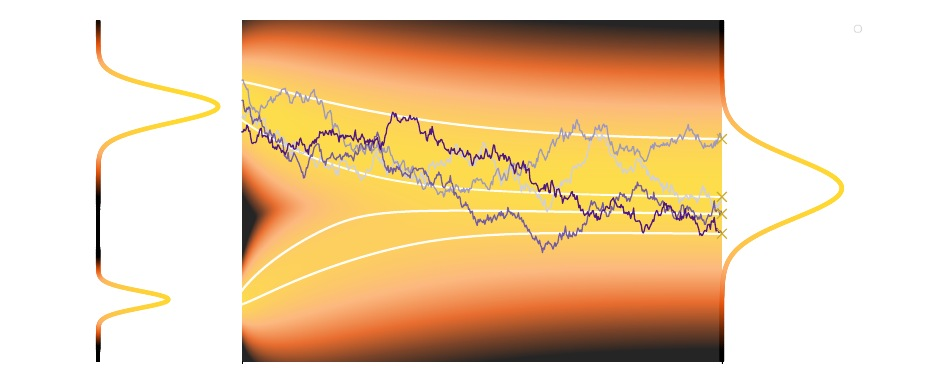
\includegraphics[width=\textwidth,height=0.62\textheight,keepaspectratio]{fig-4-4.jpg}
    \vfill
    \footnotesize
    $t=T$の事前から逆時間SDEで戻すと、$t=0$で目標の多峰分布に集まる。
\end{frame}
%=============================================
\asmain
\begin{frame}{Andersonの逆時間SDE}
    個別のブラウン軌跡は単純には逆回せないが、\\
    周辺分布の族は逆時間SDEで再現できる（Anderson, 1982）：
    \[
        \resizebox{0.98\textwidth}{!}{$
        d\bar{\bm{x}}(t)
        =
        \bigl[
        \bm{f}(\bar{\bm{x}}(t),t)
        -
        g^{2}(t)\nabla_{\bm{x}}\log p_t(\bar{\bm{x}}(t))
        \bigr]dt
        +
        g(t)\,d\bar{\bm{w}}(t)
        $}
        \tag{4.1.6}
    \]
    $\bar{\bm{x}}(T)\sim p_{\mathrm{prior}}\approx p_T$。\\
    時計$t$はデータ$=0$、ノイズ$=T$。逆向き積分では$dt<0$。
\end{frame}
%=============================================
\asmain
\begin{frame}{スコア補正が必要な理由}
    拡散$g\neq 0$があると、ドリフトをそのまま時間反転しただけでは足りない。\\
    補正項$-g^{2}(t)\nabla_{\bm{x}}\log p_t$が、前向きと同じ周辺発展を保証する。
    \begin{block}{ランジュバンとの接続（$f\equiv 0$）}
        逆時計$s=T-t$で書き直すと、温度が時間変化するランジュバン形になる。\\
        スコアは各時刻の「きれいな信号」側へ引き戻す（Tweedie）。
    \end{block}
    \begin{block}{アニーリング}
        早い段階（$t\approx T$）では$g$が大きく探索しやすい。\\
        $t\to 0$で確率的項が弱まり、高密度領域へ集中する。
    \end{block}
\end{frame}
%=============================================
\asmain
\begin{frame}{未知は時間依存スコアだけ}
    前向きの$\bm{f},g$を決めたあと、逆過程に残る未知は
    \[
        s(\bm{x},t):=\nabla_{\bm{x}}\log p_t(\bm{x})
    \]
    だけである。ネット$s_\phi(\bm{x},t)$で近似すれば（4.3で学習）、\\
    式（4.1.6）を$t=T\to 0$と解けば生成になる。
    \begin{block}{保証}
        前向きと逆向きの周辺は一致する。\\
        よって$t=0$のサンプルは$p_{\mathrm{data}}$に近い。
    \end{block}
\end{frame}
%=============================================
\asmain
\begin{frame}{逆時間SDEのまとめ}
    \begin{itemize}
        \item 生成＝事前から式（4.1.6）を逆向きに数値積分すること
        \item スコア補正$-g^{2}\nabla\log p_t$が周辺の整合を担う
        \item 学習対象は$s_\phi(\bm{x},t)\approx\nabla_{\bm{x}}\log p_t(\bm{x})$
    \end{itemize}
    \begin{block}{次}
        確率を入れない確定的な流れ（PF-ODE）もある。
    \end{block}
\end{frame}
%=============================================
\section{PF-ODEと周辺の一致}
\asmain
\begin{frame}{区切り：PF-ODEと周辺の一致}
    \tableofcontents[currentsection]
\end{frame}
%=============================================
\asmain
\begin{frame}{Question：SDEでサンプルする必要があるか？}
    逆時間SDEは確率的で多様性を出しやすいが、\\
    同じ周辺$\{p_t\}$を辿る確定的なODEも存在する。
    \begin{block}{Probability Flow ODE（PF-ODE）}
        \[
            \frac{d\tilde{\bm{x}}(t)}{dt}
            =
            \bm{f}(\tilde{\bm{x}}(t),t)
            -
            \tfrac12 g^{2}(t)
            \nabla_{\bm{x}}\log p_t(\tilde{\bm{x}}(t))
            \tag{4.1.7}
        \]
    \end{block}
    学習スコアを代入し、$t=T\to 0$と解けば生成できる。\\
    係数$\tfrac12$は「拡散項を消しただけ」ではない（Fokker--Planckから来る）。
\end{frame}
%=============================================
\asmain
\begin{frame}{PF-ODEの利点}
    \begin{columns}[T,onlytextwidth]
        \begin{column}{0.48\textwidth}
            \begin{block}{双方向}
                同じ式を$0\to T$にも$T\to 0$にも使える。\\
                （SDEは一般に前向き向きが基本）
            \end{block}
        \end{column}
        \begin{column}{0.48\textwidth}
            \begin{block}{数値解法}
                ODE用の既存ソルバがそのまま使える。\\
                高速化の議論は第9章へ。
            \end{block}
        \end{column}
    \end{columns}
    \vfill
    \begin{block}{注意}
        周辺は同じでも、サンプル軌跡の法則はSDEとODEで異なる。
    \end{block}
\end{frame}
%=============================================
\asmain
\begin{frame}{図4.5：同じ周辺、違うダイナミクス}
    \centering
    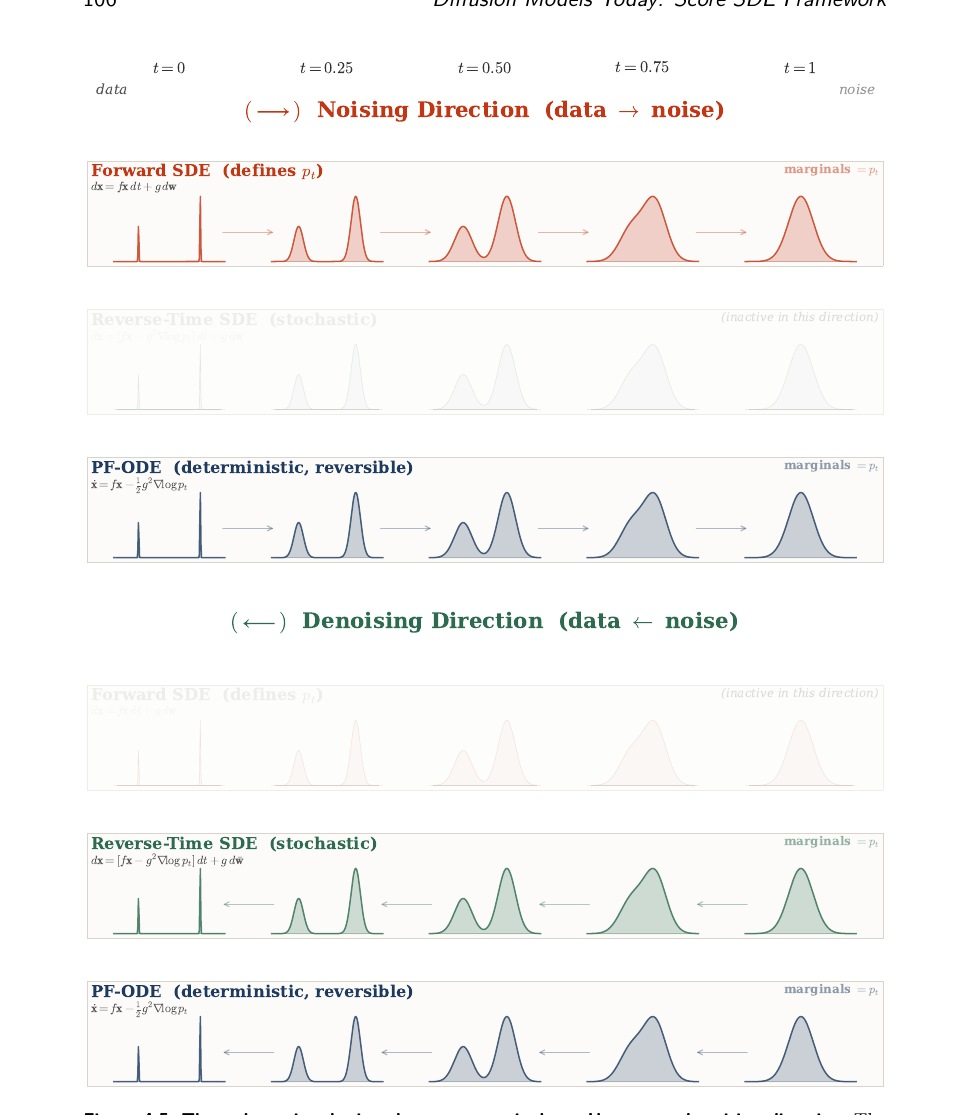
\includegraphics[width=\textwidth,height=0.68\textheight,keepaspectratio]{fig-4-5.jpg}
\end{frame}
%=============================================
\assuppl
\begin{frame}{\supplmark：図4.5の読み方}
    \begin{exampleblock}{上段（ノイズ化）}
        前向きSDEが$\{p_t\}$を定義する。\\
        PF-ODEを前向きに解いても同じ周辺列を辿る。
    \end{exampleblock}
    \begin{exampleblock}{下段（デノイズ）}
        逆時間SDEとPF-ODEを$T\to 0$で解くと、\\
        再び同じ$\{p_t\}$を逆向きに再現する。
    \end{exampleblock}
    \begin{exampleblock}{ポイント}
        スナップショットの密度が揃うことと、\\
        軌跡が同じであることとは別である。
    \end{exampleblock}
\end{frame}
%=============================================
\asmain
\begin{frame}{定理4.2.1：Fokker--Planckによる周辺の一致}
    前向きSDEの周辺$p_t$は
    \[
        \partial_t p_t(\bm{x})
        =
        -\nabla_{\bm{x}}\cdot\bigl[\bm{v}(\bm{x},t)\,p_t(\bm{x})\bigr]
        \tag{4.2.1}
    \]
    \[
        \bm{v}(\bm{x},t)
        :=
        \bm{f}(\bm{x},t)
        -
        \tfrac12 g^{2}(t)\nabla_{\bm{x}}\log p_t(\bm{x})
    \]
    を満たす。同じ$\{p_t\}$は次のどちらでも実現できる。
    \begin{enumerate}
        \item PF-ODE：$\dfrac{d\tilde{\bm{x}}}{dt}=\bm{v}$（双方向）
        \item 逆時間SDE：式（4.1.6）を$T\to 0$
    \end{enumerate}
\end{frame}
%=============================================
\asmain
\begin{frame}{Observation：周辺が揃えば生成過程は一つでなくてよい}
    \begin{block}{核心}
        大事なのはFokker--Planckを満たして$\{p_t\}$を再現すること。\\
        確率的か確定的か、どの条件付きを使うかは設計の自由度である。
    \end{block}
    \begin{itemize}
        \item 確率的核$p_t(\bm{x}_t|\bm{x}_0)$（シミュレーション不要な場合も）
        \item 確定的流$\delta\bigl(\bm{x}_t-\Psi_{0\to t}(\bm{x}_0)\bigr)$（ODEを解く）
        \item その混合なども、同じ周辺$p_t$を与え得る
    \end{itemize}
    この非一意性は、のちのFlow Matchingなどでも再登場する。
\end{frame}
%=============================================
\assuppl
\begin{frame}{\supplmark：ガウス例のスケッチ（論文4.2.2）}
    $p_{\mathrm{data}}$がガウスなら各$p_t$もガウスで、スコアが閉じる。
    \begin{exampleblock}{逆時間SDE}
        微小ステップのBayes逆遷移を$\Delta t\to 0$で展開すると、\\
        一般形（4.1.6）と同じドリフト＋拡散が得られる。
    \end{exampleblock}
    \begin{exampleblock}{PF-ODE}
        平均・分散のODEを前向きSDEと一致させるアフィン速度を選ぶと、\\
        式（4.1.7）が出る。周辺ガウスは両者で同一。
    \end{exampleblock}
    \footnotesize
    一般論（Anderson／Fokker--Planck）を、計算だけで検算できる例である。
\end{frame}
%=============================================
\asmain
\begin{frame}{PF-ODE／周辺一致のまとめ}
    \begin{itemize}
        \item PF-ODE（4.1.7）は同じ$\{p_t\}$を確定的に運ぶ
        \item Fokker--Planck（4.2.1）が「周辺が揃う」原理である
        \item 軌跡の法則は違ってよく、生成器の設計に自由度がある
    \end{itemize}
\end{frame}
%=============================================
\asmain
\begin{frame}{4.1 全体のまとめ}
    \begin{enumerate}
        \item \textbf{連続化}
        離散はしご$\to$前向きSDE（4.1.3）
        \item \textbf{生成（確率的）}
        逆時間SDE（4.1.6）。未知はスコアのみ
        \item \textbf{生成（確定的）}
        PF-ODE（4.1.7）。双方向・ODEソルバ向き
        \item \textbf{周辺}
        どちらも同じ$\{p_t\}$（Fokker--Planck／定理4.2.1）
    \end{enumerate}
\end{frame}
%=============================================
\asmain
\begin{frame}{4.1 全体のまとめ：一本の流れ}
    \begin{block}{今日の道筋}
        離散ノイズ
        $\;\to\;$
        前向きSDE
        $\;\to\;$
        スコア付き逆過程
        $\;\to\;$
        PF-ODEと周辺の一致
    \end{block}
    \begin{block}{核心}
        時間依存スコア$\nabla_{\bm{x}}\log p_t$を学べば、\\
        生成は逆時間SDEまたはPF-ODEを解く問題になる。
    \end{block}
    \begin{block}{次へ}
        4.2では、このスコアをDSMで学び、\\
        逆SDE／PF-ODEでサンプル（および尤度）する方法を見る。
    \end{block}
\end{frame}
